\section{Composing Repetition}
\label{sec:composing-repetition}

In order to unwrap the processes that eventually led to the first
version of \emph{Repetition Repeats all other Repetitions} there are
circumstances, exterior to the actual process of composing, that needs
to be considered. The first and all other encompassing is the fact
that we were both aware of and had mutually agreed on the piece being
part of a research project. Within the research project---the focus of
which was, and still is, the negotiations taking place between
different agents in composition and interpretation---we performed
theoretical studies on a collaboration between Stefan and composer
Love Mangs (as described in \citet{frisk-ost06}) in which we observed
how the constructive actions would flow back and forth between the
composer and the musician. Our analysis of this non-linear interaction
was that it played an important role in the way the music was
constructed and that the fact that the collaborators allowed it to
happen contributed to unorthodox and creative solutions to
problems. Therefore, already at the outset we agreed that the
composition, in its structure and format, should allow for external
(e.g. non-composer) input and influence---at the time of writing but
also during its phases of interpretation and performance.

As part of the agreement, and perhaps a first prerequisite for a
integrative collaboration, was also the idea of partly giving up the
traditional view on our respective roles. Specifically this means that
we consciously allowed and encouraged the `swapping of the roles' that
we had observed in the \"{O}stersj\"{o}/Mangs collaboration. As a
composer in the context of Western culture this is not a trivial thing
to partake in. The understanding of and the values traditionally
assigned to the respective labours 'composer' and 'interpreter' are
fairly rigid and socially well defined. In particular in Western art
music the composer is expected to be the authority on his own music,
its modes of expression and its meaning. To choose not to shoulder
this responsibility fully and solitarily, but rather share it and let
it be influenced by a number of factors, may easily be taken as a lack
of assurance or, worse, a sign of an unfinished, unserious or hasty
work. Similarly, an interpreter taking part in such a collaboration
may feel anxiety about trespassing into the realms of the composer.

It is notably difficult to define the end of research and the
beginning of artistic work in a project such as this and it is equally
difficult to define the type of collaboration we engage in
here. Integrative collaboration in Vera-Steiner's terminology is most
typical of artistic work, but unlike her definition we don't suspend
our differences in style. From a personal note I felt it possible to
use my background as an improviser, esthetically and stylistically,
much more fully than I have in other composition processes. As has
already been noted Complementary collaboration may be seen as typical
to performer-composer interaction but the present collaboration goes
beyond a ``division of labor''. It is more of a merging of competence
made possible due to the recursive interaction on many different
levels simultaneously. The agreed collaborative form gave us the
confidence and assurance to engage in a process that in the end
changed the object to an extent that we had not foreseen.

The other important factor to consider while tapping into this process is
the close coupling between \emph{Repetition} and a similar but
slightly larger collaboration performed within the project \emph{The
  Six Tones}. \emph{The Six Tones} was initiated in the spring 2006 at
a time when only sketches for \emph{Repetition} existed and it came to
play an important role as the two pieces were worked out in parallel
during the late summer of that year.

\subsection{The Six Tones}
\label{sec:six-tones}

In May 2006 we had the opportunity to get together with two Vietnamese
master musicians temporarily visiting Malm\"{o}: Ngo Tra My playing the
Dan Bau and Nguyen Thanh Thuy the Dan Tranh. One of the driving forces
behind engaging in this project was the attempt to go beyond a collage
like superposition of two culturally distinct musics and reach for,
not assimilation or integration but rather collocation. As freely and
unprejudiced as possible and with only loose sketches as starting
point we got together all four of us in the composition studio at the
Malm\"{o} Academy of Music to improvised. The outspoken intention was
that these sessions would provide material for a piece by Henrik for
the four of us, with Henrik on laptop.

Stefan had met with Thuy and My prior to our first playing session on
May 17 and had chosen his instruments based on the properties of the
Dan Bau and the Dan Tranh: The 10-stringed guitar would allow for a
bass register not possible on the 6-stringed guitar and the Banjo had
interesting sonic similarities with both the Dan Bau and the Dan
Tranh and blended well in with the Vietnamese instruments. As a side
note we found that the five string Banjo, seen as a result of a mix of
African and Western influences had an interesting parallel in the
Vietnamese mono chord Dan Bau, an instrument indigenous to Vietnamese
culture but adapted and amplified with modern guitar pick up
microphones.

The sketches we used as starting point for our improvising made use of
the same material I had worked out for \emph{Repetition}, at the time
merely a tone series in different permutations. For our session I had
written out one of these series as a monophonic melody line laid out
between the three string instruments as if it was one instrument
playing (see Figure X).

A number of musical ideas from these sessions (altogether we met four
times in May 2006) had a tremendous influence on how the ideas for
\emph{Repetition} evolved and how the material was composed. 
\begin{itemize}
\item Prior to the Six Tones sessions the idea was to write for
  6-stringed guitar but the register and the possibilities for
  alternate tunings made us choose the 10-string guitar instead.
\item One of the sections of \emph{Repetition} (the A-material in the
  notation) is a transcription of one of the improvisations on the
  sketch brought to the May 17 session.
\item The scordatura used in \emph{Repetition} was developed according to the needs
  presented by the \emph{Six Tones} project. (see Section XX for more
  on the scordatura.)
\item Some of the sound files used in the first version of
  \emph{Repetition} used samples recorded during the \emph{Six Tones}
  sessions.
\end{itemize}
In the end the first version of \emph{Repetition} also influenced the
first performance of and the final score for \emph{The Six Tones} in
Hanoi in October 2006. The B-material from \emph{Repetition} was
recomposed for the quartet and constitute the final section in the
version we performed.

\subsection{Composing Repetition}
\label{sec:composing-repetition-1}

With regard to the background for \emph{Repetition} yet another aspect
should be mentioned: Its inter-textual relation to \emph{Toccata
  Orpheus} by German composer Rolf Riehm. I became acquainted with
\emph{Toccata Orpheus} when Stefan and I participated in the workshop
Knowledge Lab in Berlin in June, 2005. Stefan performed the piece
(composed in 1990 for six string guitar solo) and discussed its
artistic and interpretative implications in the workshop. Following
this event we repeatedly discussed Stefan's idea of making a
multimedia performance of \emph{Toccata Orpheus} that would involve a
soundscape by me. In that process we recorded the piece in its
entirety as well as details of it for me to use as samples in the
soundscape. We also made a video recording of it that I edited and I
started elaborating on the idea of, in addition to the soundscape,
also make an electro acoustic piece with video. Though introverted in
its expression \emph{Toccata Orpheus} is a highly visual piece as the
many different and unusual playing techniques becomes part of its
construction.

When I started working on the score for \emph{Repetition} in August
2006 the Rolf Riehm piece was most certainly a source of
inspiration. Subconsciously, because I had so closely studied the piece
and discussed its possible performances with Stefan during a long
period of time. But also consciously. I was inspired by the dramaturgy
involved in the performance of the piece. In \emph{Toccata Orpheus}
the more radical and forced the movement required of the performer the
lesser the sound---in itself an interesting reversal of force. In
preparation for the soundscape mentioned above I had made an analysis
of the piece based on the movement required to perform each sound and
classified the phrases according to this analysis. I choose
to approach \emph{Repetition} in a similar manner. I borrowed Stefan's
10-stringed guitar and constructed a set of sounds based on different
playing techniques, some of which were created together with Stefan and some, such as the
two hand tapping in different tempi, which is used used extensively in
the piece and makes up the C-material, came about on his initiative.

As was mentioned above, the raw material for the piece was a simple
tone series, a version of an infinitely self-repeating series common
to much of Danish composer Per N{\o}rg{\aa}rd's music. (His Symphony
No. 3 from 1975 and Libra from 1973 are notable examples making use of
the infinity series.  The latter is recorded by Stefan in his own
transcription for 10-stringed guitar.) Conceptually the piece consists
of tree variations permutations of the same raw material, called A, B,
and C. These three motives, distinct both sonically and expressively,
are, in a manner of speaking, telling the same story in three
different ways. Though it is only possible for the guitarist to play
one of these motives at a time, irregularly moving back and forth
between them, and with the help of the computer part---also made up of
three corresponding materials, would create the illusion that all
three 'stories' were told simultaneously. The guitar and the computer
would merely 'give light' or resonate with one version of the story at
a time. The intention was to let the order of the fragments belonging
to the three motives be the result of decisions made in
performance. However, early on in the process we realized that, due to
practical reasons, with a paper score it would be impossible to employ
that level of freedom. Hence the score displayed the three materials
somewhat in parallel to each other and with written instructions about
possible choices.

In this context it should also be mentioned that my analysis software
\emph{timbreMap} already from the start of the project was intended to
constitute the link between Stefan and the computer
part. \emph{timbreMap} is a self organizing feature map that, when
fully trained, may automatically detect timbral differences in the
input audio signal. The idea was to have the software 'listen' to
Stefan and be able to detect when he moved from playing, say a
fragment of the A material to some B material. For this reason too it
was necessary for me to compose the three materials in a way that they
would be sufficiently timbrally distinct from each other for the software
to detect a change. At this time, August 2006, I had a
proof-of-concept version of \emph{timbreMap} working which gave me a
chance to evaluate and test the different playing styles and their
effect on the 'listening' computer.

\paragraph{Motive A}
\label{sec:motive}

As noted above, this motive is a transcription of the first section of
the first sketch for \emph{The Six Tones}. The transcription was made
from a recording made on May 24 which was the last of our four
sessions with My and Thuy in Malm\"{o} 2006. They both went back to
Hanoi shortly after. I made the transcription on Stefan's guitar
trying to find playing techniques that would mimic the sounds of the
two Vietnamese instruments and the Banjo, in part played with an
e-bow. Some of the playing techniques I made up and some, such as the
Koto pizzicato, were suggested by Stefan and are part of contemporary
guitar playing technique. The A motive electronics make use of samples
from the same Six Tones sessions.

\begin{figure}[htb]
  \centering
  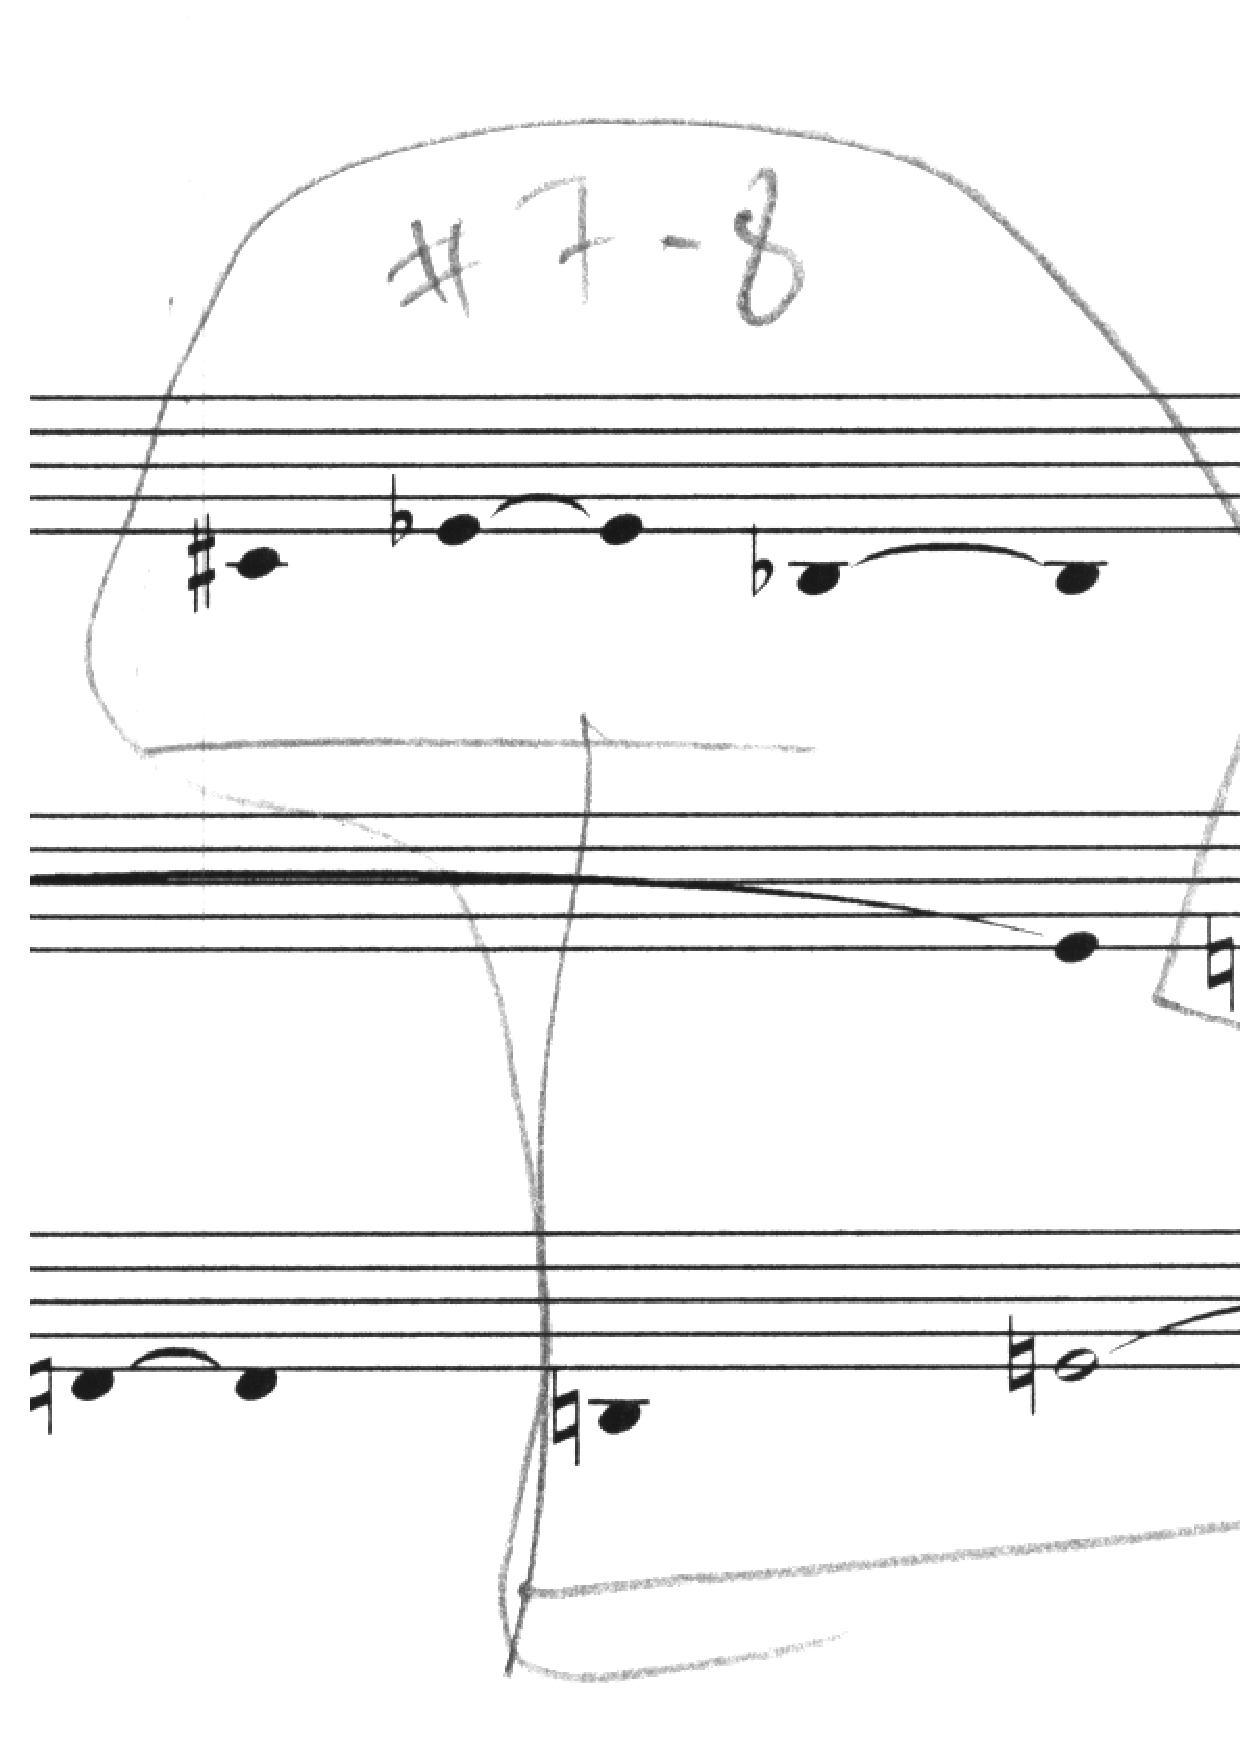
\includegraphics[width=\linewidth]{img/SixTones-transcription-1}
  \caption{An excerpt of the original sketch for \emph{The Six Tones}, the
    recording of which was used in the transcription. The numbered
    boxes correspond to the bar numbers in the score for \emph{Repetition}.}
  \label{fig:SixTones-transcription}
\end{figure}


\paragraph{Motive B}
\label{sec:motive-b}

The original idea for this motive was to present a melody derived from
the tone series all by itself. The accompanying harmony was thought to
be used in a separate section. Since the melody did not work on its
own, at least not the way I had conceived of it, and the time being to
short to realize the middle section, I decided to combine the two
elements. The harmony is likewise constructed from the tone series and
all of the chords I played myself and recorded. For the B motive
electronics I made a number of laptop improvisations with the samples
of the chords that I recorded and edited.

\paragraph{Motive C}
\label{sec:motive-c}

The C section is perhaps the most obscure of all three materials. It
is almost entirely 'tapped' on the fingerboard of the guitar using
both hands in fairly complex polyrythmic patterns. Apart from creating
a timbral texture distinct from the other two it allowed for a kind of
two line polyphony very difficult to perform playing the guitar with
standard technique. The polyrythms are derived from the harmonic ratios
between the fundamental of the tone series (the note where it
starts and in relation to which all its transpositions relate) and each
successive note (C-D has the harmonic ratio of 8:9). The computer part
plays a recording of a physical model of a guitar with glass strings
whose exciter is a recording of the C section performed by Stefan.

\subsection{Summary}
\label{sec:summary}

Looked at in isolation the production of the first version of the
score was a relatively solitary and non-collaborative process in which
I worked primarily in the poietic domain with occasional input by
Stefan, primarily in the esthesic domain. However, this version of the
score was never performed. One reason is a still unresolved practical
design related difficulty in creating an open score which allows for
the choice of the performer to be made in real time.  Furthermore
technical problems and lack of time---the first performance was only
weeks away---made it difficult to complete the interactive version of
the computer part. At the time neither I nor Stefan was probably fully
aware that this version of the score only constituted the beginning of
a long process that has yet (ever? ) to end. In hindsight it is
however clear that it is a mere raw material, exactly notated on the
detailed level but whose few performance rules regarding the greater
form we were to break in the concert versions that came out of it. The
composition process described above was in some ways the pivotal
moment, the turning point, that allowed for a transformation from a
classically conceived open work to a work-in-motion.

\subsection{The third version}
\label{sec:third-version-1}

One of the influential findings in the studies preceding the work
\emph{Repetition} was concerned with the general difference between
composer-performer interaction and performer-computer interaction. The
former is obviously bound to be more dynamic but the tolerance for the
high level of noise in the human communication was thought provoking:
Complete misunderstandings did not halt the process nor did it appear
to lead to false conclusions. If anything it seemed to be taken for
granted by both participants. It was only when looking back at the
video that the misinterpretations were identified. Our conclusion was
that what may be defined as 'noise' from the point of view of one
analytical methodology must be considered an integral part of the
artistic communication in the context of the practice. Put
differently, it shows how the classical notion of the `creative
misunderstanding' really can play an important role in artistic
processes. 

The approach to performer-computer interaction commonly taken is
however to minimize noise and to take precautions in order to avoid
it. One of the reasons for this is related to the general
understanding of a musical work in the Western Art Music tradition
(somewhat simplified): That any performer, digital or otherwise,
should follow the score exactly as written. Another reason is the
relative closeness of scientific areas such as signal processing and
information theory to electro acoustic music. In Claude E. Shannon's
influential article \emph{A Mathematical Theory of Communication}
(\citeyear{shannon48}): ``The fundamental problem of communication is
that of reproducing at one point either exactly or approximately a
message selected at another point.'' [p. 379] But as we could see from the
interactions between Stefan and Love in \citet{frisk-ost06}, in some
cases the message was not even approximately reproduced, it was
completely distorted, and yet it produced information.

There are a number of factors at play here and to simply say that
noise in the interaction may be have positive effects on the
communicative system is a too hasty conclusion. To begin with, as was
also concluded in both \citet{frisk-ost06} and \citet{frisk-ost06-2},
the subculture created by the participants in the communication system
provides a factor that reduces the entropy of the system. The
stylistic conventions of the music, the meta knowledge about the
collaborator, the other agencies involved and many other sources help
the collaborators to `understand' each other. To attempt to model and
take into account all of these constituents in a performer-computer
interactive system is not yet possible. But when designing the
interactive system it is possible to attempt to look at the message
passing as something more complex than a unidirectional stream with
the primary purpose of letting the computer know where the performer
is currently situated in time. On a technical level the interaction in
the first version (the second version is not interactive at all in
that sense---it has a prerecorded track with the computer part)
followed a traditional pedal-pressing paradigm: The temporal alignment
between performer and computer was controlled by a pedal pressed by
Stefan at times indicated in the score. The tight synchronization of
the acoustic and electronic materials has given the interaction a
certain character. These qualities have become integral to the piece
and in discussions we've had regarding the third version it has been
suggested by Stefan to keep the pedal as a complement to other means
of interaction. The musical timing may be grabbed by the computer from
the pressed pedal but the choice of event is governed by other sources
of information.

The third version is in many ways to be understood as the realisation
of the original ideas with the piece. However, since it has a long way
coming, it has also been strongly affected by the preceding
versions and by the research that have been performed by both Henrik
and Stefan, together and by themselves. As was mentioned above
\emph{Repetition} was written to be used with the timbre tracking
software \emph{timbreMap}. Based on a SOM (Self Organized Map) that
can be trained to respond similarily to two different sounds if they
share the same features provided these features were also part of the
training set. Described differently, and to connect to the
discussion above, effectively we can say that the use of
\emph{timbreMap} (or any other piece of software that implements some
kind of neural network) increases the entropy of the
system. \emph{timbreMap} `wants' and expects the input to correspond to the
the training set. In practice it will inform the system of which kind
of material Stefan is playing at the moment (A, B, or C) while the
pedal will be used for metric synchronization. A pitch
tracker that analyzes the current input and extracts its fundamental
will be used for additional information. The final level of
interaction that will be added to this version is the real-time
processing of the guitar. For instance, the physical modelling
synthesis used in the electronics for the C material will be generated
in real time rather than prerecorded.


%%% Local Variables: 
%%% mode: latex
%%% TeX-master: "../Repetition"
%%% End: 
